\documentclass[11pt]{article}

\usepackage[margin=1in]{geometry}
\usepackage{graphicx}
\usepackage{booktabs}
\usepackage{amsmath}
\usepackage{microtype}
\usepackage{xcolor}
\usepackage[colorlinks=true, linkcolor=blue!50!black, urlcolor=blue!50!black,
            citecolor=blue!50!black]{hyperref}

\newcommand{\m}[1]{$#1\,\mathrm{m}$}
\newcommand{\ms}[1]{$#1\,\mathrm{ms}$}

\title{Agent-Driven Audit and Improvement of an F1TENTH Autonomous
       Racing Stack:\\ Verified Bug Fixes and Latency-Robust
       Model-Predictive Control}
\author{AtlasAutoware contributors\thanks{Audit and implementation performed
        with Claude Code using parallel subsystem-audit and implementation
        subagents; every finding was re-verified against the code and, where
        possible, a deterministic closed-loop benchmark before adoption.}}
\date{June 12, 2026}

\begin{document}
\maketitle

\begin{abstract}
We report a systematic audit and improvement pass over AtlasAutoware, an
open-source ROS~2 racing stack for 1/10-scale (F1TENTH/RoboRacer)
autonomous racing.  Four parallel audit agents reviewed the stack's four
subsystems --- control; state estimation and planning; race strategy and
simulation bridge; and hardware drivers and perception --- producing
ranked findings that were then independently re-verified and either fixed
or rejected.  The audit surfaced eight verified defects, including three
with direct safety impact on track: a race-strategy lateral-offset clamp
with swapped wall bounds, an evasion mode that honoured a stale committed
pass side and could steer \emph{into} a passing opponent, and a two-car
simulation bridge that froze physics whenever the opponent driver
stalled.  The headline quantitative finding concerns actuator latency:
under injected sensor-to-actuator delay the model-predictive controller
(MPC) degraded severely (mean cross-track error
$0.123\,\mathrm{m} \rightarrow 0.588\,\mathrm{m}$ at $140\,\mathrm{ms}$),
and the stack's \emph{existing} delay compensation made things worse ---
it forward-simulated the newest command over the whole delay window,
while the actuator is in fact still executing the older in-flight
commands.  Replacing it with pipeline-aware prediction holds tracking at
zero-delay levels ($0.121$--$0.123\,\mathrm{m}$) across the full
$0$--$140\,\mathrm{ms}$ sweep.  A second adopted improvement removes
$0.12\,\mathrm{rad}$ steering discontinuities from the pursuit fallback's
lookup-table inversion.  Two performance hypotheses were tested and
rejected with data.  All changes are gated on a shared closed-loop metric
and covered by regression tests; the suite grew from 52 to 67 passing
tests.
\end{abstract}

\section{Introduction}

AtlasAutoware is an integrated F1TENTH racing stack: a simulation bridge
over the \texttt{f1tenth\_gym} simulator, SLAM mapping, minimum-curvature
raceline optimization with friction-limited velocity profiling, a
linear-time-varying MPC raceline tracker with an OSQP backend, a
tire-aware Model- and Acceleration-based Pursuit (MAP) fallback
controller, a lidar/camera opponent tracker feeding a race-strategy state
machine, and a hardware abstraction layer (VESC UART or PCA9685 PWM
actuation, RPLidar, OAK-D camera).  The same nodes drive both the
simulator and the physical car.

This paper documents one complete \emph{audit--verify--improve--measure}
cycle over that stack, performed by a coordinating agent orchestrating
parallel subagents.  The contributions are:
\begin{enumerate}
  \item a methodology for parallel subsystem audits with an explicit
        evidence bar for adopting changes (Section~\ref{sec:method});
  \item eight verified and fixed defects, three of them safety-relevant,
        each with a regression test where the logic is testable without
        hardware (Section~\ref{sec:bugs});
  \item a root-cause analysis and fix for the stack's actuator-delay
        compensation, with a closed-loop delay sweep, plus a smoothness
        fix to the MAP fallback's lookup-table inversion
        (Section~\ref{sec:perf});
  \item negative results: audit claims and improvement hypotheses that
        did \emph{not} survive verification, recorded so future passes do
        not re-litigate them (Section~\ref{sec:negative}).
\end{enumerate}

\section{Methodology}
\label{sec:method}

\subsection{Parallel subsystem audits}

Four read-only audit agents were launched concurrently, one per
subsystem, instructed to rank findings by impact~$\times$~confidence and
to verify suspicions by executing the stack's pure-logic paths (the
repository isolates its mathematics from ROS, so controllers, estimators,
planners, and protocol codecs all run under plain \texttt{pytest}):

\begin{itemize}
  \item \textbf{Control}: LTV-MPC (\texttt{mpc\_controller.py}), its ROS
        wrapper with AEB and traction governor
        (\texttt{raceline\_mpc.py}), the MAP pursuit fallback, and the
        pure-pursuit agent.
  \item \textbf{Estimation and planning}: velocity EKF with slip
        rejection, lidar de-skew, friction-ellipse velocity profiler,
        minimum-curvature raceline optimizer and OSQP refiner,
        Frenet-frame overtaking spliner.
  \item \textbf{Strategy and simulation bridge}: opponent tracker and
        sensor fusion, race-strategy state machine
        (\texttt{race\_brain.py}), two-car gym bridge.
  \item \textbf{Hardware and perception}: drive node (watchdog, arming,
        backend autodetect), VESC UART protocol, PCA9685 PWM driver,
        RPLidar binning, camera perception geometry.
\end{itemize}

\subsection{Evidence bar}

Audit findings are treated as \emph{hypotheses}.  Each was re-verified
against the source by the coordinating agent before any code change;
claims that could not be reproduced were rejected
(Section~\ref{sec:negative}).  Behavioural changes had to satisfy two
gates:
\begin{enumerate}
  \item \textbf{Regression gate}: the full unit/closed-loop test suite
        passes, and each fixed defect gains a test that fails on the old
        code wherever the logic is hardware-independent.
  \item \textbf{Benchmark gate}: performance-motivated changes must
        improve the shared deterministic closed-loop lap benchmark
        (Section~\ref{sec:harness}) and may not regress the zero-delay
        baseline.
\end{enumerate}

Verified single-site defects were fixed by the coordinating agent.  The
two controller-level work items were implemented by two parallel
subagents with strictly disjoint file ownership, so no two agents wrote
to the same file; their claims (including ``adopted'' vs.\ ``rejected''
calls) were then re-run and re-verified by the coordinator before
committing.

\subsection{The shared closed-loop harness}
\label{sec:harness}

All quantitative claims use the repository's single benchmark
(\texttt{tests/closed\_loop.py}): a kinematic-bicycle plant integrated at
$50\,\mathrm{Hz}$ lapping the competition raceline
(\texttt{racelines/comp\_raceline.csv}, 300 points, profiled speeds
$1.6$--$7.0\,\mathrm{m/s}$), starting from a deliberate
$0.36\,\mathrm{m}$ pose error.  The harness reports lap time and
perpendicular cross-track error (XTE; mean and max after a settle
period), and can hold each command in a FIFO to emulate
sensor-to-actuator latency.  The plant matches the model the MPC plans
with, so results isolate \emph{controller} behaviour from model error;
runs are deterministic and free of ROS scheduling noise.

\section{Verified defects and fixes}
\label{sec:bugs}

Table~\ref{tab:bugs} summarises the eight verified defects.  Three
deserve narrative treatment.

\begin{table}[t]
  \centering
  \small
  \begin{tabular}{@{}p{2.0cm}p{4.6cm}p{4.0cm}p{3.6cm}@{}}
    \toprule
    Subsystem & Defect & Failure mode on track & Fix \\
    \midrule
    Strategy &
    All four lateral-offset clamps used swapped wall bounds:
    $\mathrm{clip}(\delta, -\mathrm{room}_L, +\mathrm{room}_R)$ for a
    $+$left offset $\delta$ &
    Lateral moves limited by the \emph{opposite} wall's free room; wall
    contact exactly when clamping matters &
    Clamp to $[-\mathrm{room}_R, +\mathrm{room}_L]$ \\
    \addlinespace
    Strategy &
    EVADE honoured the pass side committed during a previous attack &
    Evading \emph{into} the car that is now passing &
    Always move away from the opponent; clear the stale commitment \\
    \addlinespace
    Sim bridge &
    Two-car physics stepped only when \emph{both} drivers had published &
    Simulation freeze on any opponent-side stall; ego plans against
    ghost-car scans &
    Step on ego publish, opponent uses its last-known command \\
    \addlinespace
    Drive node &
    Watchdog disarmed until the first \texttt{/drive} message ever
    arrived (\texttt{last\_cmd${}=0$} vs.\ a \texttt{${}>0$} guard) &
    No command-timeout neutral before the first command &
    Arm the watchdog at startup \\
    \addlinespace
    Drive node &
    Watchdog \texttt{neutral()} exceptions swallowed silently &
    Operator unaware the car did \emph{not} go neutral &
    Log the failure (throttled) \\
    \addlinespace
    Drive node &
    VESC UART steering used the full $\pm0.5$ servo span, ignoring the
    configured half-range &
    One side's full lock clipped whenever trim${}\neq 0$ (UART backend
    only); asymmetric steering &
    Mirror the PCA9685 map: centre${}+{}$trim${}+{}$frac${}\cdot{}$half-range \\
    \addlinespace
    VESC protocol &
    \texttt{parse\_values} read fixed offsets with no length guard &
    \texttt{struct.error} in the telemetry loop on a truncated payload &
    Length check; return \texttt{None} \\
    \addlinespace
    PCA9685 &
    \texttt{us\_to\_ticks} unclamped &
    Overflow into the always-ON register bit for over-long pulses &
    Clamp to the 12-bit range \\
    \bottomrule
  \end{tabular}
  \caption{Verified defects.  Each has a regression test except the
  simulation-bridge fix (it requires a live two-car simulator); that fix
  is a guard-condition change reviewed in place.  Two hygiene items were
  fixed alongside: invalid lidar beams are zeroed before the de-skew
  rotation (silencing a numpy \texttt{RuntimeWarning}; output unchanged),
  and the lap-counter wrap zone now scales with raceline density.}
  \label{tab:bugs}
\end{table}

\paragraph{Swapped wall clamps.}
The strategist expresses lateral offsets in metres, positive to the
\emph{left} of the raceline; $\mathrm{room}_L$ and $\mathrm{room}_R$ are
lidar-measured free distances to the left and right walls.  Every clamp
in the decision function read $\mathrm{clip}(\delta, -\mathrm{room}_L,
+\mathrm{room}_R)$ --- i.e.\ a left move was limited by the \emph{right}
wall's room.  With a wall \m{0.1} to the left and open track to the
right, a DEFEND decision would command a \m{0.35} left offset ---
\m{0.25} into the wall.  The bug is invisible on wide track (both rooms
large), and bites exactly when clamping matters.  Found at all four
decision sites (attack, slipstream, evade, defend).

\paragraph{Stale evasion side.}
Once the strategist commits to a pass side it remembers it (hysteresis
--- correct, otherwise the attack oscillates between sides).  But the
alongside-and-being-passed branch (EVADE) reused that committed side.
Sequence: ego commits to pass left; the opponent instead accelerates and
draws alongside on the left; EVADE then offsets \emph{left} --- into the
opponent, at closing speed.  The fix computes the away-side dynamically
in EVADE and clears the stale commitment; a regression test drives the
full two-phase scenario and asserts the offset sign flips away from the
passer.

\paragraph{Frozen two-car physics.}
The bridge stepped the simulator only when \emph{both} cars' drivers had
published since the last tick.  Any opponent-side stall (startup
ordering, a crashed node, a GC pause) silently froze the world --- while
the sensor-publishing timer kept republishing the last observation, so
the ego raced against a ghost car.  Physics now steps as soon as the ego
has published, using the opponent's last-known command (neutral before
its first message) --- which is also the semantics a real race has: the
world does not wait for anyone's software.

\section{Performance: latency-robust MPC and fallback smoothness}
\label{sec:perf}

\subsection{Actuator-delay compensation: root cause and fix}
\label{sec:delay}

A real car has $50$--$150\,\mathrm{ms}$ of sensor-to-actuator latency
(serial links, servo lag, ESC ramping).  The baseline sweep
(Table~\ref{tab:delay}, ``naive'') shows the MPC --- which tracks to
\m{0.123} mean XTE at zero delay --- degrading $4.8\times$ by
\ms{140}, with lap time inflating from $41.5$ to $69.5\,\mathrm{s}$.

The stack already shipped a compensator: \texttt{predict\_state}
forward-integrates the kinematic bicycle by the known delay and the MPC
solves from the predicted pose.  Benchmarked closed-loop, however, the
shipped compensation was \emph{worse than no compensation} at \ms{80}
(XTE mean $0.242$ vs.\ $0.195$) and unstable beyond \ms{100}: at
\ms{120}--\ms{140} it produced corner-cutting laps with XTE means above
\m{0.5}.  The root cause is the prediction's command semantics: it held
the \emph{newest} commanded (steer, speed) constant over the whole delay
window.  But under pipeline latency the actuator is still executing the
\emph{older in-flight} commands during that window --- the newest command
has not reached the wheels yet.  Whenever steering is changing (every
corner entry and exit) the prediction over-rotates the pose, and the
error grows with delay until the loop destabilizes.

The fix keeps a buffer of the commands published during the last delay
window and integrates the prediction through them oldest-first, each
holding its slice of the window (\texttt{mpc\_controller.py},
\texttt{raceline\_mpc.py}; scalar inputs keep bit-identical legacy
behaviour for existing callers).  Table~\ref{tab:delay} and
Figure~\ref{fig:delay} show the result: tracking holds at zero-delay
levels --- XTE mean $0.121$--$0.123\,\mathrm{m}$, lap time within
$0.12\,\mathrm{s}$ of baseline --- across the entire $0$--\ms{140}
sweep.  A regression test gates the \ms{100} case (compensated lap must
complete with XTE mean below \m{0.2}).

\begin{table}[t]
  \centering
  \small
  \begin{tabular}{@{}r rrr rrr rrr@{}}
    \toprule
    & \multicolumn{3}{c}{Naive (no compensation)}
    & \multicolumn{3}{c}{Shipped compensation}
    & \multicolumn{3}{c}{Pipeline-aware (fixed)} \\
    \cmidrule(lr){2-4}\cmidrule(lr){5-7}\cmidrule(l){8-10}
    Delay (ms) & lap (s) & $\overline{\mathrm{XTE}}$ & max
               & lap (s) & $\overline{\mathrm{XTE}}$ & max
               & lap (s) & $\overline{\mathrm{XTE}}$ & max \\
    \midrule
      0 & 41.48 & 0.123 & 0.406 & 41.48 & 0.123 & 0.406 & 41.48 & 0.123 & 0.406 \\
     40 & 40.40 & 0.111 & 0.354 & 41.52 & 0.121 & 0.403 & 41.52 & 0.122 & 0.405 \\
     80 & 43.74 & 0.195 & 0.538 & 42.08 & 0.242 & 0.652 & 41.54 & 0.122 & 0.405 \\
    100 & 50.48 & 0.322 & 0.804 & 42.16 & 0.261 & 0.599 & 41.56 & 0.121 & 0.404 \\
    120 & 59.86 & 0.461 & 1.108 & 33.72$^{\dagger}$ & 0.508 & 1.472 & 41.58 & 0.121 & 0.404 \\
    140 & 69.52 & 0.588 & 1.381 & 33.90$^{\dagger}$ & 0.539 & 1.496 & 41.60 & 0.121 & 0.404 \\
    \bottomrule
  \end{tabular}
  \caption{Closed-loop MPC under injected actuator delay
  (\texttt{tools/benchmark\_delay.py}; XTE in metres).  The shipped
  compensation simulated the newest command over the whole delay window
  and was worse than naive at $80\,\mathrm{ms}$;
  $^{\dagger}$\,its short ``laps'' at $120$--$140\,\mathrm{ms}$ are
  corner-cutting, not speed.  The pipeline-aware fix holds zero-delay
  tracking across the sweep.}
  \label{tab:delay}
\end{table}

\begin{figure}[t]
  \centering
  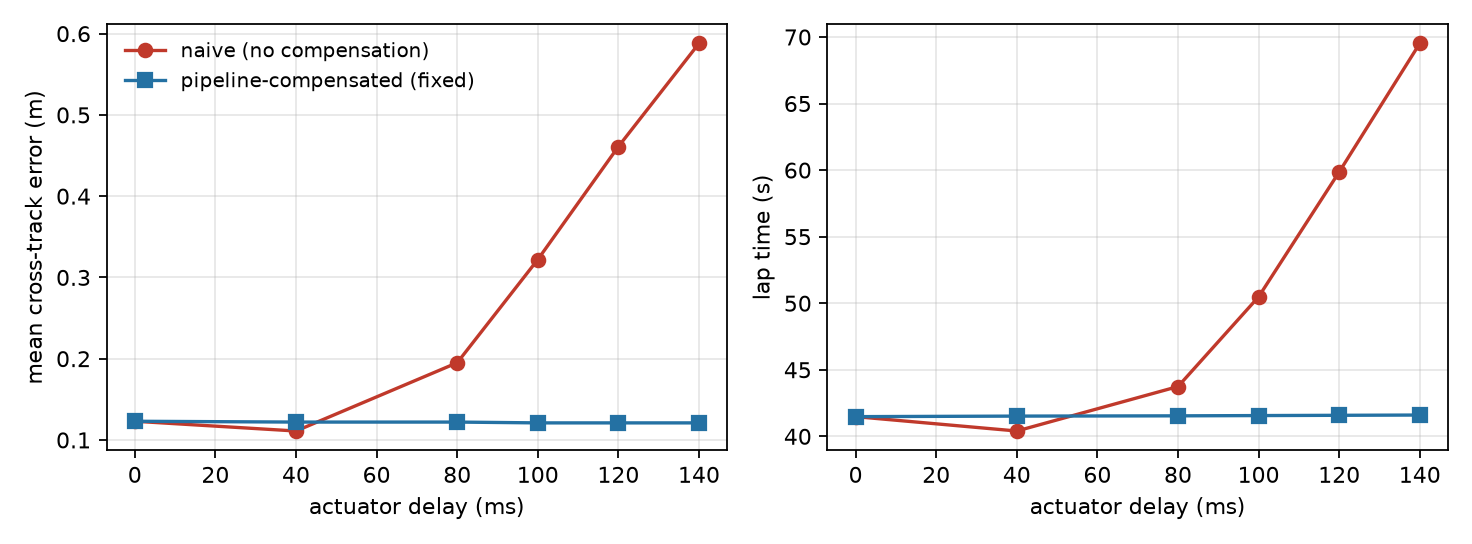
\includegraphics[width=\textwidth]{figures/mpc_delay_sweep.png}
  \caption{MPC tracking under actuator delay, naive vs.\ pipeline-aware
  compensation (compensator told the true delay).  Left: mean
  cross-track error; right: lap time.  The compensated controller is
  flat across $0$--$140\,\mathrm{ms}$.}
  \label{fig:delay}
\end{figure}

\subsection{MAP fallback: speed-axis interpolation of the steer LUT}

The MAP fallback inverts a lateral-acceleration$\,\to\,$steer lookup
table.  The lateral-acceleration axis was interpolated, but the speed
axis selected the \emph{nearest} LUT column, so the commanded steering
jumped by up to $0.119\,\mathrm{rad}$ ($\approx 6.8^{\circ}$) every time
speed crossed a column midpoint (Figure~\ref{fig:lut}).  The fix inverts
the two bracketing speed columns and blends linearly --- bit-identical at
the LUT's sample speeds, clamped to the edge columns outside the table,
and \emph{cheaper} per call ($\approx 5\,\mu\mathrm{s}$) because each
column's monotonic inversion branch is precomputed once.

Closed-loop, the change is neutral-to-slightly-better at all profile
scalings (at $1.3\times$ speed: XTE mean $0.1575 \rightarrow 0.1564$,
max $1.287 \rightarrow 1.267$, steering-rate std
$1.144 \rightarrow 1.104\,\mathrm{rad/s}$); it was adopted for the
open-loop continuity, which matters on the physical car where each
discontinuity excites the steering servo.  Nine unit tests pin the new
behaviour (continuity in $v$, betweenness, oracle match at sample
speeds, clamps, odd symmetry).

\begin{figure}[t]
  \centering
  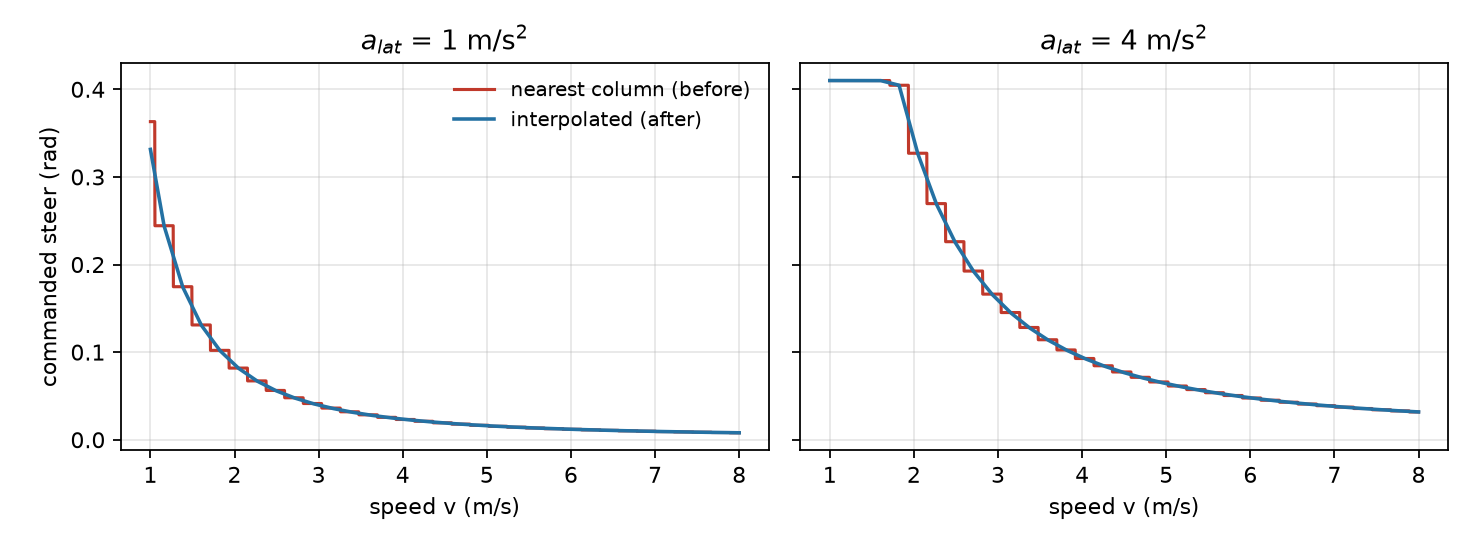
\includegraphics[width=\textwidth]{figures/map_lut_interpolation.png}
  \caption{MAP controller commanded steer vs.\ speed at constant lateral
  acceleration.  Nearest-column lookup (red) steps at every column
  midpoint --- worst jump $0.119\,\mathrm{rad}$ at
  $a_{lat}=1\,\mathrm{m/s^2}$; the bracketing-column interpolation
  (blue) is continuous.}
  \label{fig:lut}
\end{figure}

\section{Negative results}
\label{sec:negative}

Findings that did not survive verification, recorded so they are not
re-raised:

\begin{itemize}
  \item \textbf{Estimation and planning are clean.}  The audit of the
        velocity EKF (Jacobians, Joseph-form covariance update, slip
        gating), the lidar de-skew geometry, the friction-ellipse
        forward--backward velocity profiler (including propagation
        across the lap seam), the minimum-curvature optimizer/refiner QP
        formulations, and the Frenet spliner found \emph{no correctness
        defects}; the only action was the cosmetic NaN-warning fix.
  \item \textbf{MPC formulation is sound.}  The control audit checked
        the discrete linearization, angle unwrapping, OSQP warm-start
        usage, and the persistent-QP sparsity-update path, and confirmed
        them correct.
  \item \textbf{``Nearest index not recomputed after prediction''
        --- false.}  The control audit hypothesized the ROS node fed the
        MPC a nearest-raceline index computed from the stale
        (un-predicted) pose.  Inspection showed the node already
        recomputes it from the predicted pose; the delay defect was the
        command-pipeline semantics of Section~\ref{sec:delay}.
  \item \textbf{``Reference temporal mismatch under delay'' ---
        rejected empirically.}  After the pipeline fix, residual
        compensated XTE ($0.121$) matches the zero-delay baseline
        ($0.123$), leaving nothing for a reference-time shift to
        explain.
  \item \textbf{Curvature-scaled speed weighting --- rejected.}
        Scaling the MPC's speed-tracking weight by reference curvature,
        $q_v\,(1 + k\,|\kappa_{\mathrm{ref}}|)$, was implemented via
        per-tick OSQP \texttt{Px} updates and swept over
        $k \in \{0.5, 1, 2, 4\}$: XTE mean rose monotonically
        ($0.123 \rightarrow 0.125$--$0.134$) with no
        $\mathrm{XTE}_{\max}$ improvement at any gain.  On a kinematic
        plant with no grip limit, harder speed-profile tracking only
        trades away position tracking.  The implementation was reverted;
        the experiment is recorded in \texttt{docs/mpc.md}.
  \item \textbf{AEB time-to-collision is ego-speed based.}  The audit
        flagged that lidar AEB computes TTC from the ego's closing
        component only, underestimating risk for head-on traffic.  Real,
        but it is the standard single-lidar formulation (no per-beam
        range rate); a proper fix needs opponent velocity fused into the
        AEB path and is scoped as future work rather than a landed
        half-measure.
\end{itemize}

\section{Threats to validity}

The harness plant is the same kinematic bicycle the MPC plans with:
results isolate controller logic but exclude tire slip, which on the
real car is handled by the separate traction governor and slip-rejecting
EKF (audited clean, unchanged here).  Delay compensation is evaluated
with the compensator told the true delay; on hardware the delay must be
identified and set (\texttt{actuation\_delay} parameter), and the
sensitivity of the pipeline-aware predictor to a misidentified delay is
not characterized here.  The strategy fixes are validated by unit-level
scenario tests, not full two-car simulation, which requires the ROS/gym
environment unavailable in the audit sandbox.  Closed-loop XTE
differences below ${\sim}0.005\,\mathrm{m}$ are within the harness's
discretization noise and are not claimed as improvements.

\section{Conclusion}

A parallel agent audit of a mature, well-tested racing stack (52 passing
tests at baseline) still surfaced three safety-relevant logic defects ---
all in code paths that only execute near walls, alongside opponents, or
under partner-node failure, exactly where unit suites are thinnest.  The
quantitative lesson is sharper: the controller tracked to \m{0.12} in
the zero-latency benchmark while its \emph{deployed} path --- delay
compensation included --- was unbenchmarked, and that compensation
turned out to be worse than nothing at realistic latencies because it
simulated a command the wheels had not yet received.  Racing stacks
should benchmark the deployed control path, latency included, not the
idealized solver --- and keep one deterministic closed-loop metric that
every change, and every plausible-sounding improvement hypothesis, must
face.  Of the four improvement hypotheses tested here, two were adopted
and two rejected; the rejections are as much a part of the audit record
as the fixes.

\appendix
\section{Reproduction}

All numbers in this paper are reproducible from the repository root:

\begin{verbatim}
python3 -m pytest tests/ -q          # full suite (67 tests)
python3 tests/test_mpc.py            # closed-loop MPC validation
python3 tools/benchmark_delay.py     # delay sweep (Table 2, Figure 1)
python3 tools/benchmark_map.py       # MAP LUT closed-loop comparison
python3 tools/benchmark_lookahead.py # pursuit lookahead scheduling
python3 tools/benchmark_refiner.py   # raceline refinement lap times
\end{verbatim}

\end{document}
